\documentclass[12pt]{article}
\usepackage[utf8]{inputenc}
\usepackage{polski}
\usepackage[a4paper, left=2.0cm, right=2.0cm, top=2.0cm, bottom=2.0cm]{geometry}
\usepackage{graphicx}
\usepackage{multicol}


\title{PIISW, W08, IO, 2021/2022, semestr letni\\Lista zadań nr 2: JavaScript}
\author{mgr inż. Maciej Małecki\\\small{maciej.malecki@pwr.edu.pl}}

\begin{document}
    \maketitle

    \section*{Zasady oddawania zadań}
        \begin{enumerate}
            \item Zadania z~tej listy mogą być oddawane \emph{wyłącznie} za pośrednictwem prywatnego repozytorium na portalu \texttt{github.com}.
            \item Przed zajęciami, na których oddawana będzie lista należy nadać prowadzącemu uprawnienia do odczytu dla w.w. repozytorium.
            \item Rozwiązanie każdego z~zadań musi znaleźć się w~katalogu o~nazwie \texttt{zad-x} gdzie \texttt{x} jest numerem zadania.
            \item Rozwiązanie każdego z~zadań musi mieć nazwę \texttt{index.html}.
            \item Proszę o~wykorzystywanie jedynie standardowego API przeglądarki, w~szczególności zabronione jest korzystanie z~bibliotek typu JQuery.
            \item Każde rozwiązanie powinno działać po otwarciu w.w. pliku w~przeglądarce Chrome (chyba, że w~zadaniu zaznaczono inaczej).
        \end{enumerate}

    \section*{Oceny}
    \begin{tabular}{|l|c|c|c|c|c|c|}
        \hline
        Punkty: & $<9$ & $9-10$ & $11-12$ & $13-14$ & $15-16$ & $17-18$\\
        \hline
        Ocena:  & $2,0$ & $3,0$ & $3,5$ & $4,0$ & $4,5$ & $5,0$\\
        \hline
    \end{tabular}

    \section*{Zadania}
        \begin{enumerate}
        \item\label{exc:dom-model}
            (5 pkt) Obsługa zdarzeń modelu DOM.

            Utwórz dokument HTML z~osadzonymi stylami oraz z~osadzonym kodem JavaScript, który wyświetli dwa elementy: kontrolkę suwaka oraz koło.

            \begin{enumerate}
                \item Przyjmij zakres dopuszczalnych wartości suwaka jako $10 - 500$.
                \item Średnica koła powinna być zawsze równa wartości ustawionej na suwaku (w~pikselach).
                \item Średnica koła powinna zmieniać się dynamicznie podczas przesuwania suwaka.
                \item Wewnątrz koła, w~jego geometrycznym środku powinna być zawsze wyświetlana jego średnica.
                \item Podpowiedź: koło można wyświetlić z~pomocą odpowiednio ostylowanego elementu \texttt{div}.
            \end{enumerate}

            Przykład wyglądu strony dla dwóch wybranych pozycji suwaka przedstawiono na rysunku~\ref{fig:dom-model}.

            \begin{figure}[p]
                \centering
                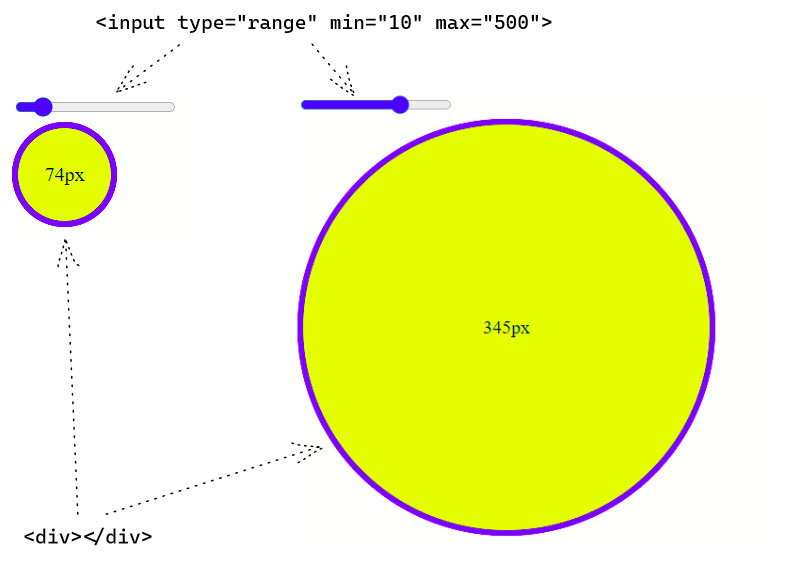
\includegraphics[width=0.8\textwidth]{lista-2-1}
                \caption{Dwie fazy działania kodu z~zadania~\ref{exc:dom-model}.}
                \label{fig:dom-model}
            \end{figure}

    \end{enumerate}
\end{document}

